% ============================================================
% file: pinn_residual_three_graphs_simple.tex
% Three computational graphs: u, u_x, u_xx
% Network: y = wx, z = wx + b, u = sigma(z)
% Residual: r = u_xx + a u_x
% ============================================================

\documentclass{standalone}
\usepackage{tikz}
\usetikzlibrary{arrows.meta, positioning, calc}
\usepackage{amsmath}
\usepackage{amssymb}

\begin{document}

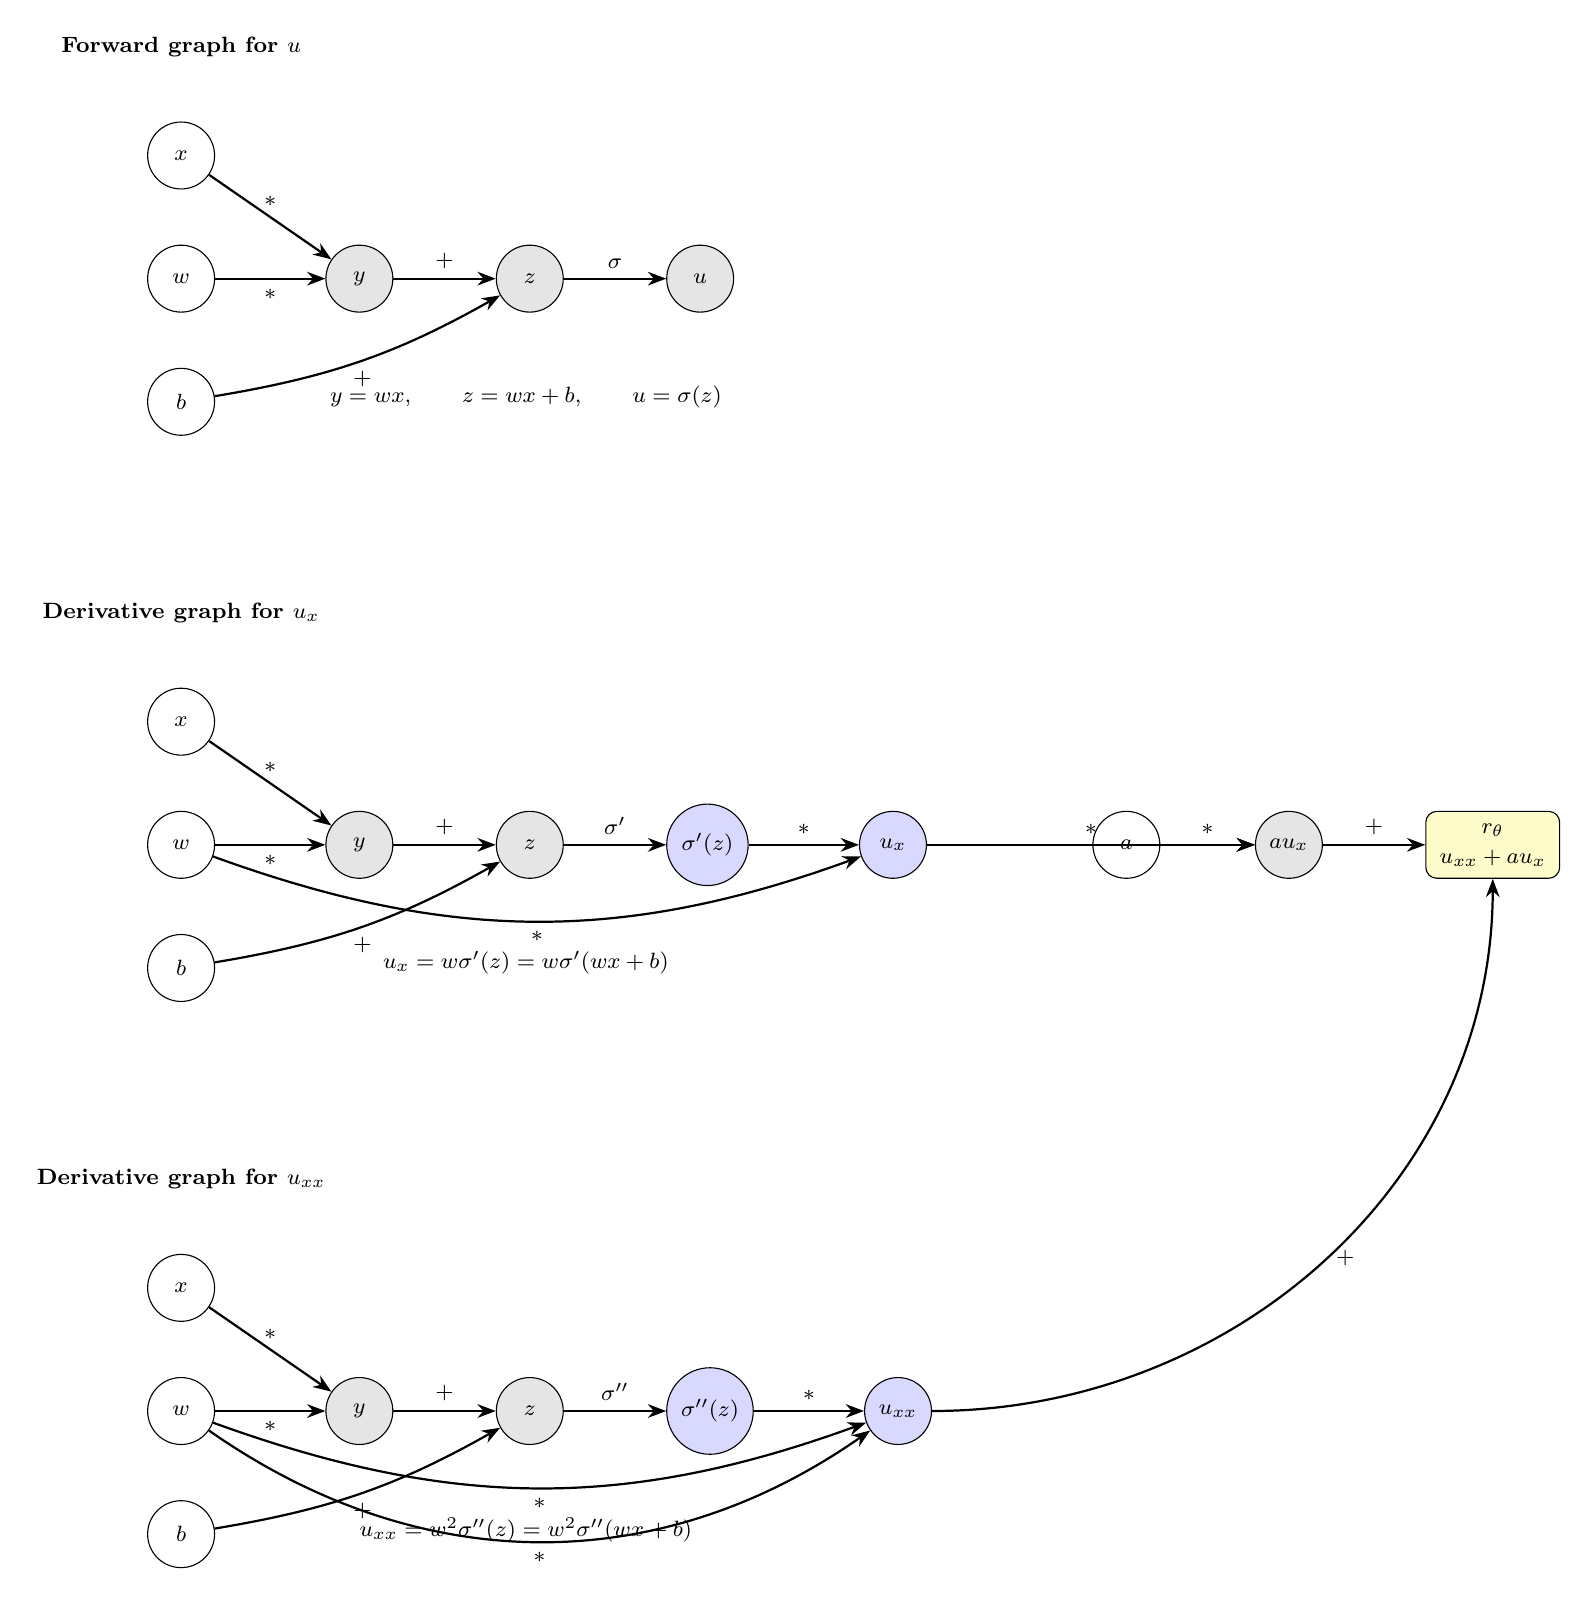
\begin{tikzpicture}[
  node/.style={
    circle,
    draw,
    minimum width=0.85cm,
    minimum height=0.85cm,
    align=center,
    fill=gray!20
  },
  leaf/.style={
    node,
    fill=white!20
  },
  deriv/.style={
    node,
    fill=blue!15
  },
  residual/.style={
    rectangle,
    draw,
    rounded corners,
    minimum width=1.7cm,
    minimum height=0.85cm,
    align=center,
    fill=yellow!20
  },
  every node/.style={font=\footnotesize},
  arrow/.style={-Stealth, thick}
]

% ============================================================
% Graph 1: u
% ============================================================

\node[align=center] (titleu) {\textbf{Forward graph for $u$}};

\node[leaf, below=0.7cm of titleu] (x1) {$x$};
\node[leaf, below=0.7cm of x1] (w1) {$w$};
\node[leaf, below=0.7cm of w1] (b1) {$b$};

\node[node, right=1.4cm of w1] (y1) {$y$};
\node[node, right=1.3cm of y1] (z1) {$z$};
\node[node, right=1.3cm of z1] (u1) {$u$};

\draw[arrow] (x1) -- node[above] {$*$} (y1);
\draw[arrow] (w1) -- node[below] {$*$} (y1);

\draw[arrow] (y1) -- node[above] {$+$} (z1);
\draw[arrow] (b1) to[bend right=10] node[below] {$+$} (z1);

\draw[arrow] (z1) -- node[above] {$\sigma$} (u1);

\node[align=center, below=0.8cm of z1] {
$y=wx,\qquad z=wx+b,\qquad u=\sigma(z)$
};

% ============================================================
% Graph 2: u_x
% ============================================================

\node[align=center, below=2.0cm of b1] (titleux) {\textbf{Derivative graph for $u_x$}};

\node[leaf, below=0.7cm of titleux] (x2) {$x$};
\node[leaf, below=0.7cm of x2] (w2) {$w$};
\node[leaf, below=0.7cm of w2] (b2) {$b$};

\node[node, right=1.4cm of w2] (y2) {$y$};
\node[node, right=1.3cm of y2] (z2) {$z$};
\node[deriv, right=1.3cm of z2] (sp) {$\sigma'(z)$};
\node[deriv, right=1.4cm of sp] (ux) {$u_x$};

\draw[arrow] (x2) -- node[above] {$*$} (y2);
\draw[arrow] (w2) -- node[below] {$*$} (y2);

\draw[arrow] (y2) -- node[above] {$+$} (z2);
\draw[arrow] (b2) to[bend right=10] node[below] {$+$} (z2);

\draw[arrow] (z2) -- node[above] {$\sigma'$} (sp);
\draw[arrow] (sp) -- node[above] {$*$} (ux);
\draw[arrow] (w2) to[bend right=20] node[below] {$*$} (ux);

\node[align=center, below=0.8cm of z2] {
$u_x=w\sigma'(z)=w\sigma'(wx+b)$
};

% ============================================================
% Graph 3: u_xx
% ============================================================

\node[align=center, below=2.0cm of b2] (titleuxx) {\textbf{Derivative graph for $u_{xx}$}};

\node[leaf, below=0.7cm of titleuxx] (x3) {$x$};
\node[leaf, below=0.7cm of x3] (w3) {$w$};
\node[leaf, below=0.7cm of w3] (b3) {$b$};

\node[node, right=1.4cm of w3] (y3) {$y$};
\node[node, right=1.3cm of y3] (z3) {$z$};
\node[deriv, right=1.3cm of z3] (spp) {$\sigma''(z)$};
\node[deriv, right=1.4cm of spp] (uxx) {$u_{xx}$};

\draw[arrow] (x3) -- node[above] {$*$} (y3);
\draw[arrow] (w3) -- node[below] {$*$} (y3);

\draw[arrow] (y3) -- node[above] {$+$} (z3);
\draw[arrow] (b3) to[bend right=10] node[below] {$+$} (z3);

\draw[arrow] (z3) -- node[above] {$\sigma''$} (spp);
\draw[arrow] (spp) -- node[above] {$*$} (uxx);
\draw[arrow] (w3) to[bend right=20] node[below] {$*$} (uxx);
\draw[arrow] (w3) to[bend right=35] node[below] {$*$} (uxx);

\node[align=center, below=0.8cm of z3] {
$u_{xx}=w^2\sigma''(z)=w^2\sigma''(wx+b)$
};

% ============================================================
% Residual: r = u_xx + a u_x
% ============================================================

\node[leaf, right=2.1cm of ux] (a) {$a$};
\node[node, right=1.2cm of a] (aux) {$a u_x$};

\node[residual, right=1.3cm of aux] (res) {
$r_\theta$\\[0.05cm]
$u_{xx}+a u_x$
};

\draw[arrow] (ux) -- node[above] {$*$} (aux);
\draw[arrow] (a) -- node[above] {$*$} (aux);

\draw[arrow] (aux) -- node[above] {$+$} (res);
\draw[arrow] (uxx.east) to[out=0,in=-90] node[right] {$+$} (res.south);

\end{tikzpicture}

\end{document}